\section{Dispositif: Effet Tcherenkov par des muons}
\label{sect:Tcherenkov_muon}

L'effet Tcherenkov survient lorsqu'une particule chargée se déplace plus vite que la vitesse de la lumière dans un milieu diélectrique. Ce phénomène résulte de la superposition cohérente d'onde électromagnétique suite à la polarisation du milieu par le passage de la particule chargée. Si la vitesse de la particule est supérieure au ratio $c/n$ (où $n$ est l'indice de réfraction et $c$ la vitesse de la lumière dans le vide), il y a formation d'un cône de lumière avec un angle de demi-ouverture $\theta_c$ qui suit la relation:
\begin{equation}
    cos\theta_c = \frac{1}{n\beta}
\end{equation}\\
où $\beta = v/c$, $v$ étant la vitesse de la particule dans le milieu. Le nombre de photons Tcherenkov émis par unité de longueur et de longeur d'onde est donné par la formule de Frank-Tamm:
\begin{equation}
     \frac{d^2N}{dx \, d\lambda} = \frac{2\pi \, \alpha}{\lambda^2} \; (1- \frac{1}{n^2 \, \beta^2} )
\end{equation}\\
avec $\alpha$ étant la constante de structure-fine. Comme le nombre de photons produits est inversement proportionnel à la longueur d'onde, la contribution des petites longueurs d'onde est plus importante.

Compte tenu de leur faible section efficace d'interaction, la détection des neutrinos nécessite un détecteur de grand volume. Cela est réalisé par les détecteurs Tcherenkov en déployant des photo-multiplicateurs (PMs) dans un volume de matériau diélectrique. Chaque PM est contenu dans une bulle de verre sous vide, l'ensemble étant appelé module optique (OM). AMANDA (Antarctic Muon and Neutrino Detector Array) est un télescope à neutrino localisé au Pôle Sud. Lors de sa phase finale, le détecteur était composé de 677 modules optiques (OMs) disposés sur 19 câbles. Ces modules retourne un signal analogique. Après 9 ans d'activité, AMANDA a été officiellement incorporé au détecteur IceCube en 2005. IceCube (figure~\ref{fig:IceCube}) est un détecteur Tcherenkov d'un kilomètre cube enterré dans la glace du Pôle Sud. Il a pour but principal la détection des neutrinos à haute énergie. IceCube est composé de 5160 modules optiques digitaux (DOMs ou Digital Optical Modules) placés sur 86 câbles. Pour constituer un vaste réseaux d'OMs, il nous faut connaître la réponse de chacun de ceux-ci.

\begin{figure}
    \center{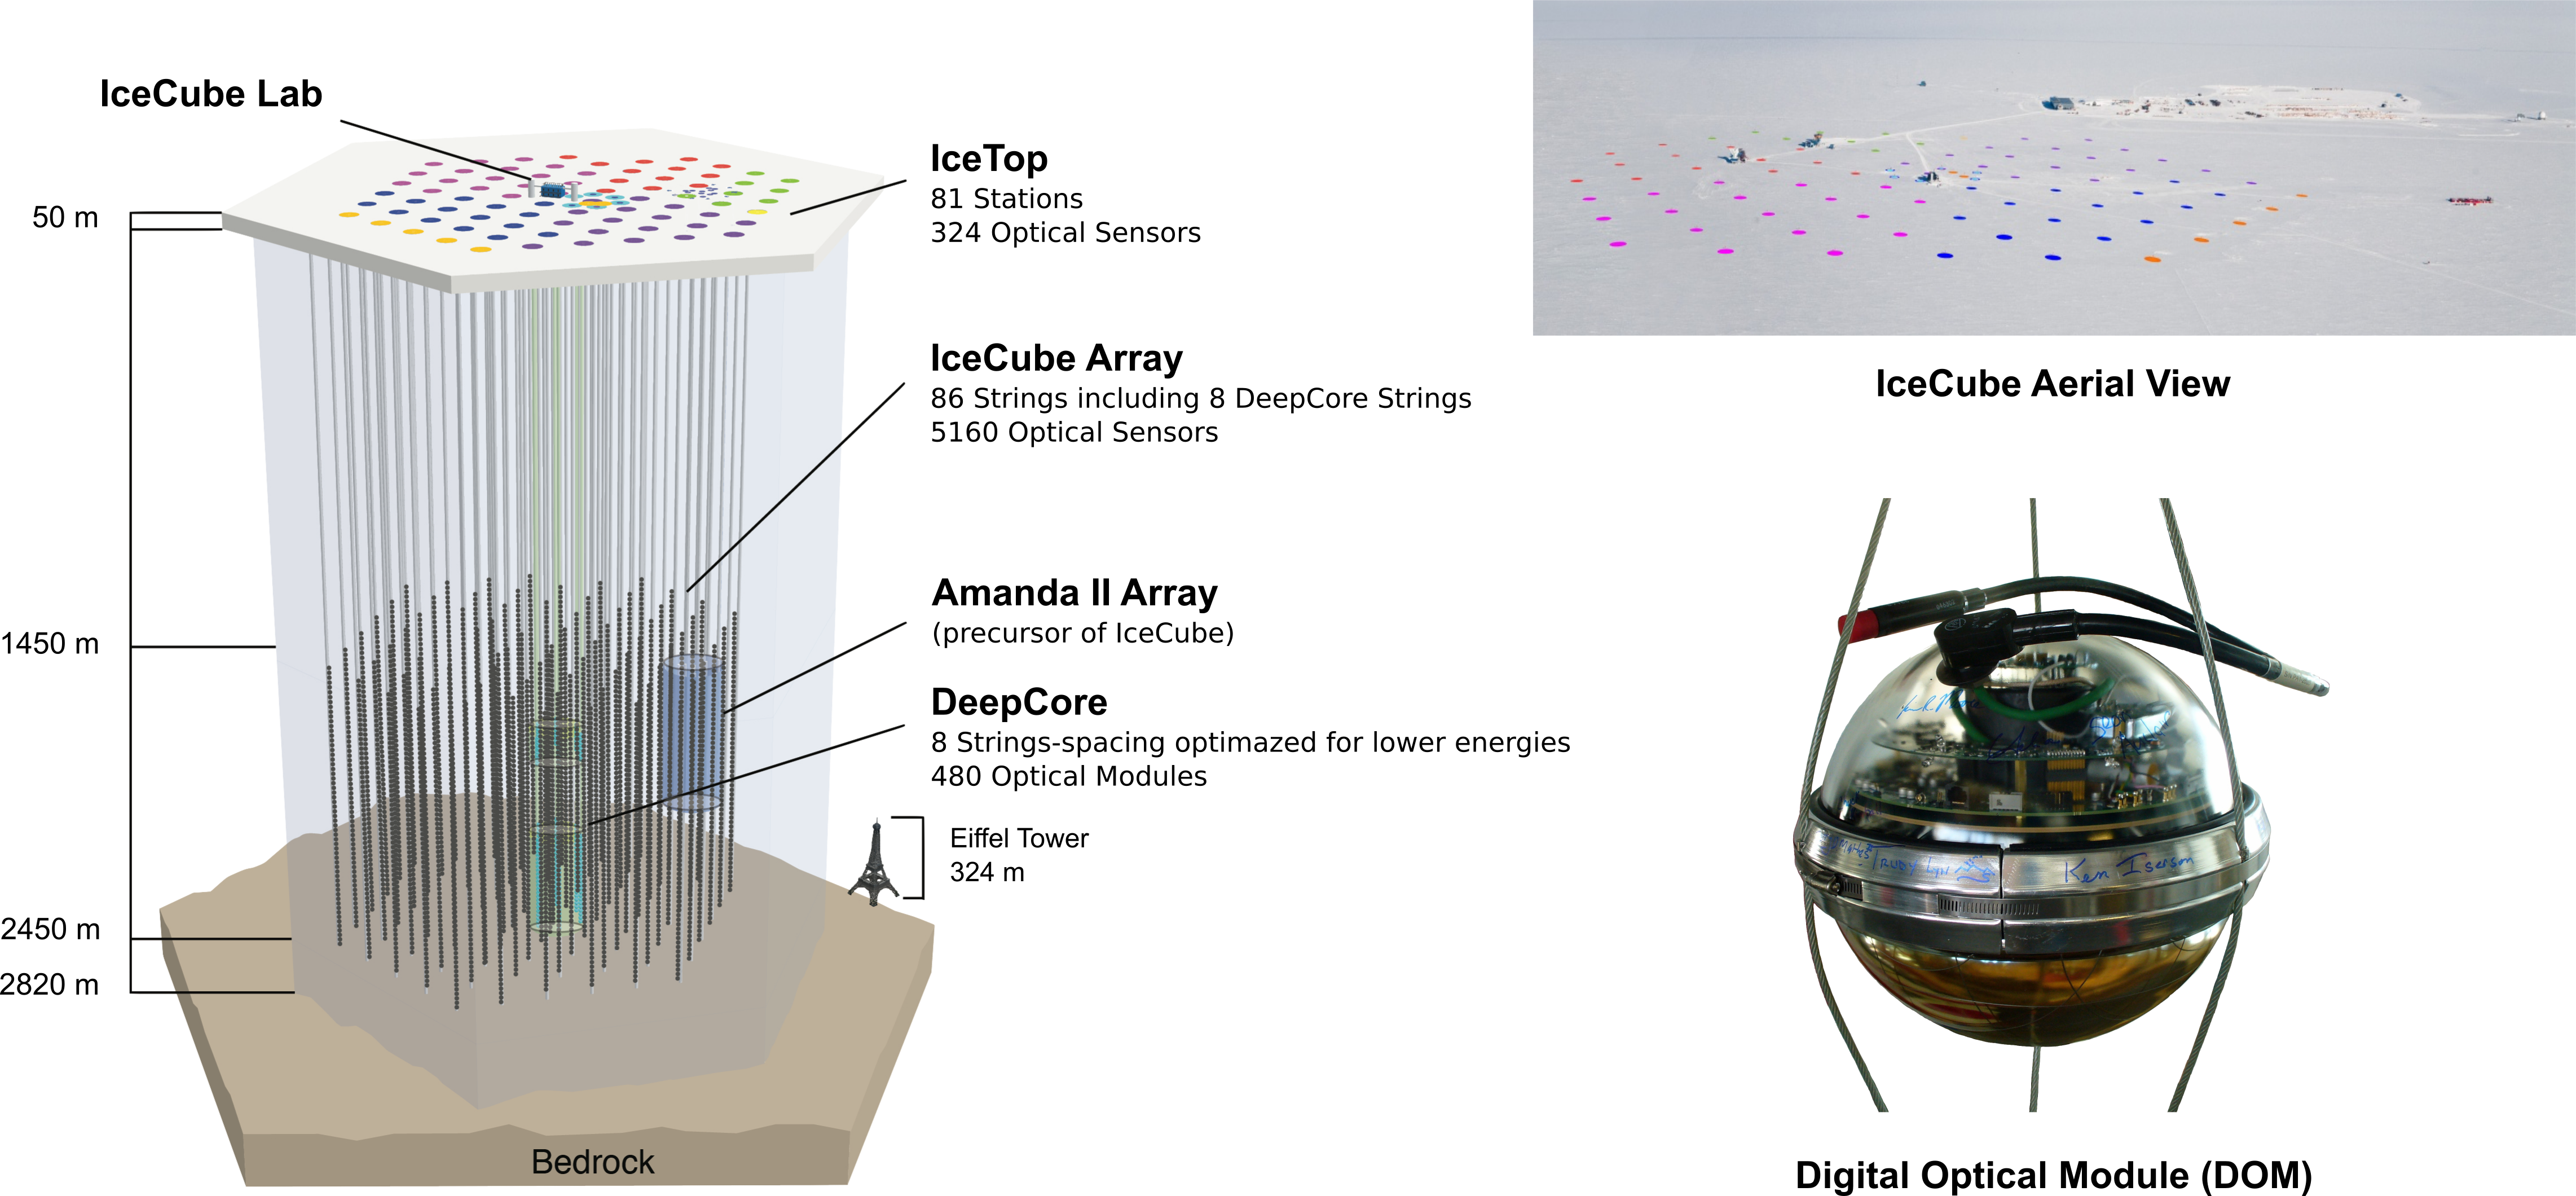
\includegraphics[width=0.8\textwidth]
    {figures/IceCube_Detector.png}}
    \caption{\label{fig:IceCube} Configuration du télescope à neutrinos IceCube.}
\end{figure}

Cette manipulation a pour but la caractérisation d'un module optique (OM) développé pour l'expérience AMANDA. Afin d'étudier les propriétés de cet OM, vous devrez mettre au point le dispositif nécessaire à la prise de mesure. Après avoir pris connaissance avec le dispositif, vous serez ainsi amené à développer vous même la logique d'acquisition des données. Vous analyserez ensuite les données recueillies grâce aux outils statistiques et informatiques que vous aurez vu en cours.

\subsection{Agenda du laboratoire}
\begin{tabular}{p{0.2\linewidth} p{0.8\linewidth}}
Lundi & - Prise de connaissance avec le matériel\newline
		- Vérification du signal analogique des PMs avec l'oscilloscope\newline
		- Implémentation de la table de vérité pour la logique d'acquisition ou trigger\newline
		- Mesure de l'efficacité\\ 

Mardi & - Calibration de l'ADC\newline
		- Préparation de l'acquisition de données\newline
		- Début de l'acquisition de données avec LabView\\ 

Mercredi & - Construction de la logique d'acquisition du bruit de fond\newline
		- Écriture de la table de vérité pour définir un événement du bruit\newline
		- Début de l'acquisition de données pour le bruit de fond\\ 

Jeudi et Vendredi & - Développement d'un programme de génération MC d'une distribution normale\newline
		- Développement des programmes d'analyse\newline
		- Dernier jour pour présenter les résultats des exercices\newline
		- Préparation de la présentation\\
\end{tabular} 

\subsection{Dispositif expérimental}

Pour cette manipulation, nous utilisons les muons atmosphériques afin d'obtenir l'émission Tcherenkov. Ce dispositif est composé de 4 scintillateurs chacun relié à un photo-multiplicateur (PM), d'un OM, une couche de plomb et d'un réservoir d'eau (voir figure \ref{fig:dispo2}). Ce réservoir forme un angle de 45$^{\circ}$ avec la verticale. Les trois premiers PMs (PM1, PM2 et PM3) assurent la direction verticale du muon incident. La présence d'une couche de plomb avant le PM3 nous permet également de vérifier que le muon est suffisamment énergétique pour produire le rayonnement Tcherenkov avec l'angle souhaité. Un 4ème PM est placé au dessus de l'OM et est utilisé comme veto. Puisque les muons sont produits en "paquets", appelés muon bundles, ce veto exclu les évènements de l'OM qui seraient produits par un second muon plutôt que par un photon Tcherenkov.

\begin{figure}
    \centering
	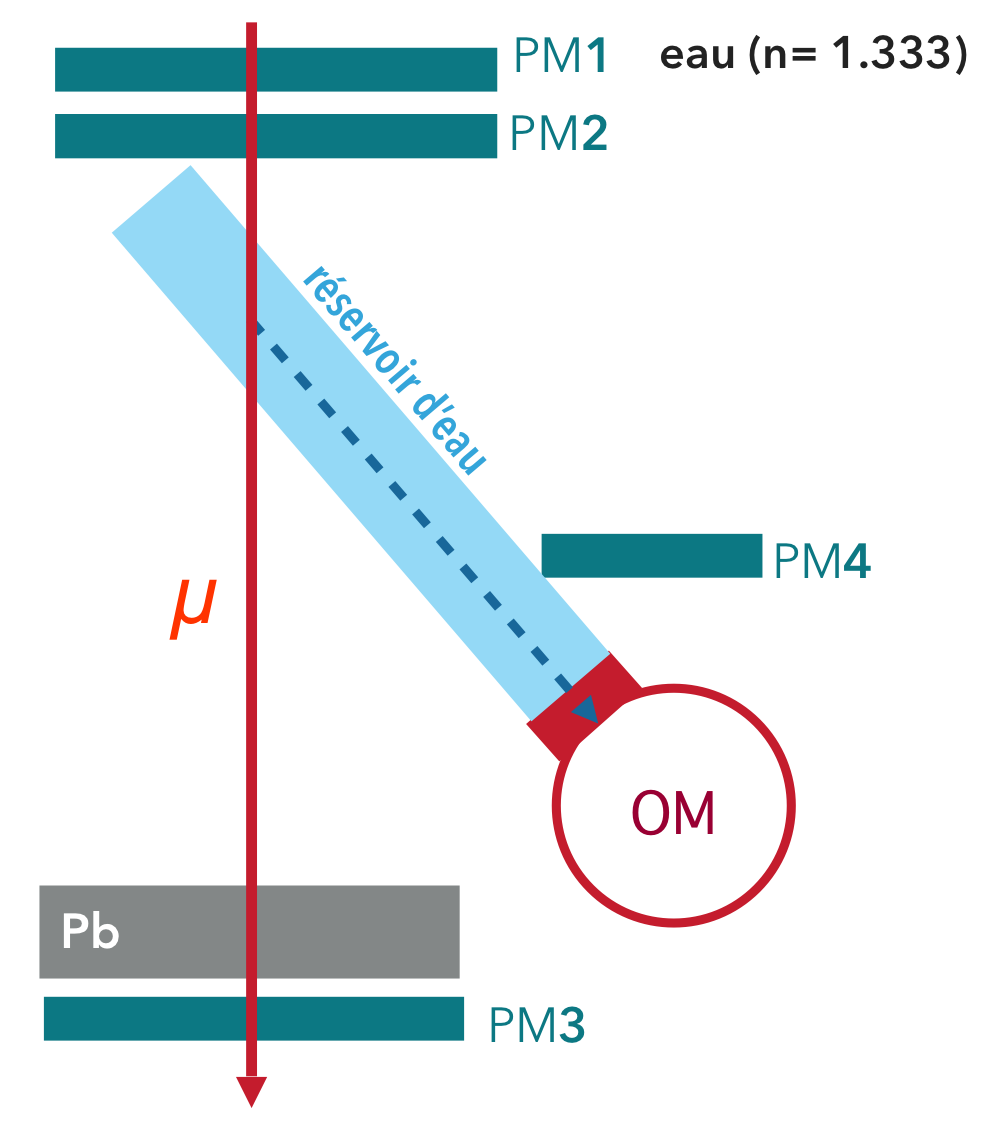
\includegraphics[width=0.5\textwidth]{figures/Dispositif_2.png}
    \caption{Dispositif expérimental de l'effet Tcherenkov produit par des muons.}
    \label{fig:dispo2} 
\end{figure}

\subsection{Exercices Pr\'eparatoires}

\subsubsection{Exercice 1}
Calculez quelle sera l'angle d'\'emission du rayonnement Tcherenkov \'emis dans l’eau par des muons ($m_\mathrm{\mu} = 0.106$\,GeV/$c^2$) de $1.5$\,GeV/$c$ de quantité de mouvement, sachant que l'indice de r\'efraction de l'eau \`a $20^\circ$C est $1.333$.

\ifthenelse{\boolean{showAdditional}}{
\begin{additional}
\begin{align*}
\begin{split}
\beta &= \frac{v}{c} = \frac{pc}{E}\\
 &= \frac{pc}{\sqrt{p^2c^2+m_\mathrm{\mu}^2c^4}}\\
 &= 0.9975\\
\end{split}
\quad
\begin{split}
\cos\Theta_\mathrm{c} &= \frac{1}{\beta n}\\
 \Theta_\mathrm{c} &= \arccos\frac{1}{0.9975\cdot1.33}\\
 &= \boxed{41.2^\circ} 
\end{split}
\end{align*}
\end{additional}
}

\subsubsection{Exercice 2}
\textbf{We should modify this to the muon setup!}\\
Pour le 1er dispositif, calculer l'ordre de grandeur du nombre de photons \'emis entre $350$ et $500$\,nm par un 'electron de $1247$\,keV d'\'energie cin\'etique traversant une fen\^etre de quartz de 1\,mm d'\'epaisseur, sachant que pour ce domaine de longueurs d’onde, l'indice de r\'efraction du quartz varie de moins de 1\% et peut \^etre consid\'er'e constant ($1.478$). N\'egliger la perte d'\'energie de l'\'electron dans le quartz.\\ $\alpha = 1/137$

\ifthenelse{\boolean{showAdditional}}{
\begin{additional}
Formule de \emph{Frank-Tamm}:
\begin{align*}
\frac{\mathrm{d}N}{\mathrm{d}x} &= \int_{\lambda_0}^{\lambda_1} \frac{2\pi\alpha z^2}{\lambda^2} \sin^2\Theta_\mathrm{c} \mathrm{d}\lambda\\
&=\frac{\pi}{137}\int_{350\,\mathrm{nm}}^{500\,\mathrm{nm}}\frac{\mathrm{d}\lambda}{\lambda^2}\\
N&=\frac{\pi}{137}\cdot\left(\frac{1}{350\,\mathrm{nm}}-\frac{1}{500\,\mathrm{nm}}\right)\cdot1\,\mathrm{mm}\\
&=\boxed{19.65}
\end{align*}
\end{additional}
}

\subsubsection{Exercice 3}
\textbf{We should modify this to the muon setup!}\\
En supposant que le diam\`etre du collimateur plac\'e devant la photocathode de l'OM est de 6 cm et qu'il se trouve \`a 17\,cm de la fen\^etre de quartz, combien de photoelectrons l'OM peut-il enregistrer par \'electron de la source, en supposant la transmittance $T$ \`a 90\%, l'efficacit\'e quantique est de $\epsilon_\mathrm{q}=15\%$?

\ifthenelse{\boolean{showAdditional}}{
\begin{additional}
Avec $N_\mathrm{\gamma}^{\mathrm{quartz}}$ trouv\'e avant, on obtient:
\begin{align*}
N_{\mathrm{pe}} &= \epsilon_\mathrm{q} \cdot T \cdot N_\mathrm{\gamma}^{\mathrm{OM}}\\
 &= \epsilon_\mathrm{q} \cdot T \cdot \frac{6\,\mathrm{cm}}{2\pi \cdot 17\,\mathrm{cm} \cdot\sin\Theta_\mathrm{c}} \cdot N_\mathrm{\gamma}^{\mathrm{quartz}}\\
&= \boxed{3.58}
\end{align*}
\end{additional}
}

\subsection{Prise de mesure}

Pour cette manipulation, il vous est demandé de préparer le dispositif expérimental nécessaire à la prise de mesure. Cela implique, dans un premier temps, de :\\

\begin{center}
\fbox{
\begin{minipage}{0.75\textwidth}
\textbf{Se familiariser avec le dispositif :} 
\begin{quote}
\begin{itemize}
\item vérifier le signal des différents PMs et de l'OM
\item étudier l'efficacité des PMs
\item calibrer l'ADC
\item développer la logique d'acquisition de données
\item mesurer le bruit de fond
\end{itemize}
\end{quote}
\end{minipage}
}
\end{center}

\subsubsection{Vérification du dispositif}
Dans un premier temps, allumez votre dispositif et allumez la haute tension aux bornes des PMs. Veillez ne pas changer la tension indiquée afin de ne pas endommager les PMs.\\
A l'aide de l'oscilloscope, vérifiez le signal provenant des différents photo-multiplicateurs (PMs) et de l'OM. Transformez ensuite votre signal analogue en signal digital à l'aide du discriminateur et observez celui-ci sur l'oscilloscope.

\subsubsection{Mesure de l'efficacité}

Il vous est ensuite demandé de mesurer l'efficacité d'un des PMs présents dans votre dispositif. Vous devrez faire cette mesure en faisant varier dans un premier temps le seuil du PM pour lequel vous mesurer l'efficacité. Une fois la valeur optimale du seuil trouvée, répétez le processus en faisant cette fois varier la tension appliquée sur le PM en question. Pour ces deux mesures, veillez également à mesurer le taux d'évènements détectés par le PM dont vous mesurez l'efficacité. Pour effectuer ces mesures, vous avez à votre disposition un scaler NIM. De quel PM allez-vous mesurer l'efficacité ?

\ifthenelse{\boolean{showAdditional}}{
\begin{additional}
\begin{itemize}
\item Mesure de l'efficacité de PM2
\item Logique : (PM1 \& PM2 \& PM3) et (PM1 \& PM3)
\item Mesure du rate de PM2
\end{itemize}
\end{additional}
}

\subsubsection{Calibration de l'ADC}

Nous allons à présent procéder à la calibration du convertisseur analogique-numérique (ADC ou Analogue-to-Digital Converter). En effet, l'ADC vous donne des valeurs en ADC channel, il vous faut donc connaître à quelle charge équivaut un ADC channel.

Pour cette calibration, il faut fournir une charge connue et constante à l'ADC. Pour cela, vous avez à votre disposition un générateur de courant continu. Comment allez-vous procéder ? 

\ifthenelse{\boolean{showAdditional}}{
\begin{additional}
\begin{itemize}
    \item Charge de l'ADC de l'ordre du pC $\to$ $Q\sim100$\,pC 
    \item Utilisation d'une résistance: $U = RI$ avec $R = 2.2$\,k$\mathrm{\Omega}$
    \item Sachant que $Q = I\mathrm{\Delta}t$, déterminer $\mathrm{\Delta}t$
    \item Le gate est ensuite créé à l'aide du dual-timer
\end{itemize}
\end{additional}
}

\subsubsection{Prise de données}

Afin de prendre les données nécessaires à la caractérisation de l'OM, nous devons réfléchir à la logique d'acquisition. Nous allons utiliser l'ADC que nous venons de calibrer et lui fournir le signal de l'OM ainsi qu'une porte logique (gate). Pour créer ce gate, nous avons besoin des modules logiques. Il nous faut réfléchir aux conditions dans lesquelles ont veut déclencher la prise de mesure. En d'autres termes, quand-est-ce que le signal de l'OM nous intéresse? Une fois que cela est clair, vous pouvez l'implémenter à l'aide des modules logiques. Il vous faudra ensuite vérifier que le signal de l'OM et votre porte logique sont en coïncidence à l'aide de l'oscilloscope. Lorsque vous avez effectué cette vérification, reliez le gate et le signal de l'OM à l'ADC pour commencer la prise de mesure.

\textbf{Attention :} Pour la manipulation utilisant les muons, veillez à changer le nom du fichier pour ne pas qu'il soit écrasé lors de la prise de mesure suivante.

\ifthenelse{\boolean{showAdditional}}{
\begin{additional}
\begin{itemize}
\item \textbf{Gate :} (PM1 \& PM2 \& PM3) \& (OM \& !PM4)
\item Faire passer le gate dans le dual-timer pour avoir des fenêtres de taille constante
\item Vérifier que l'OM est en même temps que le gate
\item On veut aussi le muon rate ($\sim 1$\,Hz) donc on passe (PM1 \& PM2 \& PM3) dans le scaler relié au PC
\item Donner le gate et le signal à l'ADC (taux de coïncidence $\sim 0.2$\,Hz) et commencez la prise de mesure
\end{itemize}
\end{additional}
}

\subsubsection{Mesure du bruit de fond}

Intéressons nous au bruit de fond présent dans votre manipulation. Nous voulons connaître le taux de fausses coïncidences, càd les cas où l'OM nous envoie un signal qui n'est pas dû à un photon Tcherenkov alors que notre porte logique s'est déclenchée.

Dans un premier temps, il vous faut réfléchir à la manière dont vous pouvez implémenter la prise de mesure du bruit de fond. Une fois cette méthode mise en place, vous pouvez démarrer l'acquisition du bruit de fond. A l'aide de l'oscilloscope, pensez toutefois à vérifier que le signal de l'OM et votre gate arrivent en même temps à l'ADC.

\ifthenelse{\boolean{showAdditional}}{
\begin{additional}
\begin{itemize} 
\item \textbf{Gate :} (PM1 \& PM2 \& PM3) \& (OM$_{\mathrm{delayed}}$) \& !(PM4)
\begin{quote}
    A l'aide d'un câble, on ajoute un délai de 50\,ns sur l'OM avant la logique\\
    Cela permet la mesure du taux de fausses coïncidences\\
    On obtient un taux très faible avec $\sim 1$ évènement par heure
\end{quote}

\item \textbf{Gate :} !(PM1 \& PM2 \& PM3) \& (OM) \& !(PM4)
\begin{quote}
    On s'intéresse ici à tous les évènements de l'OM qui ne sont pas dû à un photon Tcherenkov\\
    A partir de cela, on peut néanmoins calculer le taux de fausses coïncidences\\
    $R_{\mathrm{fc}} = 2 \cdot R_{\mathrm{mu}} \cdot R_{\mathrm{bf}} \cdot f $ \\
    où $R_{\mathrm{fc}}$ est le taux de fausse coïncidence, $R_{\mathrm{\mu}}$ le taux de muons et $f$ est la fenêtre de temps.
\end{quote}
\end{itemize}
\end{additional}
}

\subsection{Analyse de donn\'ees}

A présent, nous pouvons nous concentrer sur l'analyse des données dans le but de caractériser l'OM.

En vous basant sur les données, vous devrez calculer:\\
\begin{center}
\fbox{
\begin{minipage}{0.75\textwidth}
\textbf{Dispositif muon :}
\begin{itemize}
\item le gain $G$ de l'OM,
\item la r\'esolution $\sigma_\mathrm{G}$ de l'OM,
\item le nombre moyen de photo-\'electrons $\langle n_{\mathrm{pe}}\rangle$ produit par trigger dans l'OM.
\end{itemize}
\end{minipage}
}
\end{center}

\ifthenelse{\boolean{showAdditional}}{
\begin{additional}
\textbf{Validation de la procedure d'adjustement:}\\
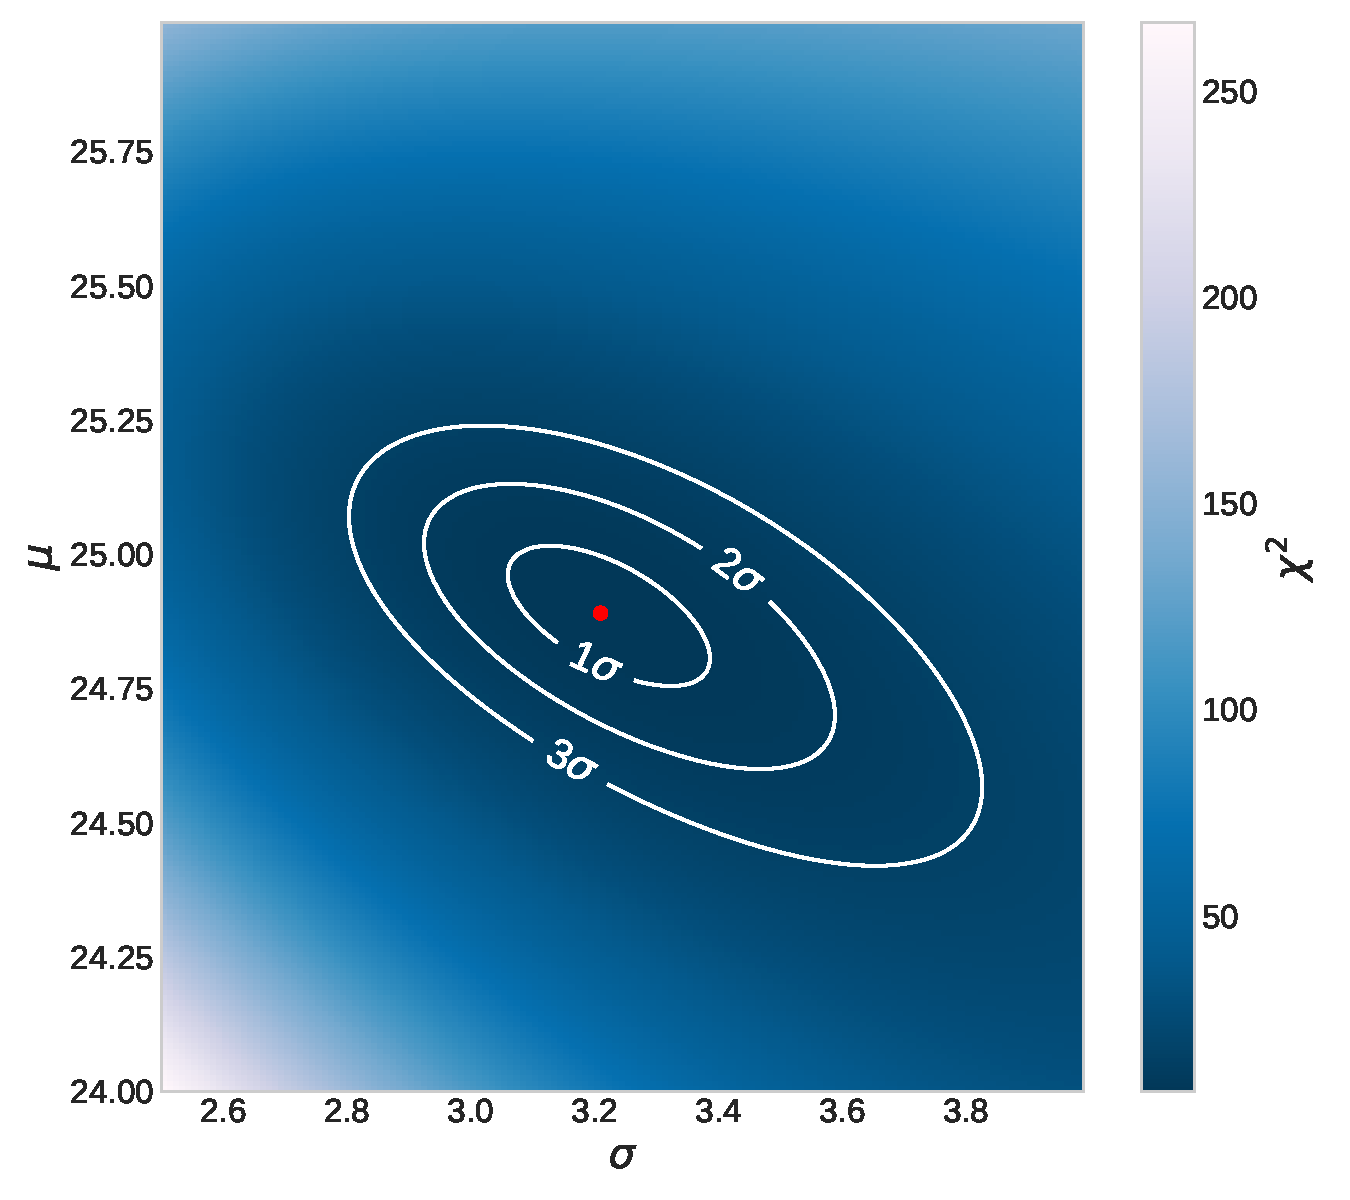
\includegraphics[width=0.45\textwidth]{exampleAnalysis/plots/Chi2_MC.pdf}
\hfill 
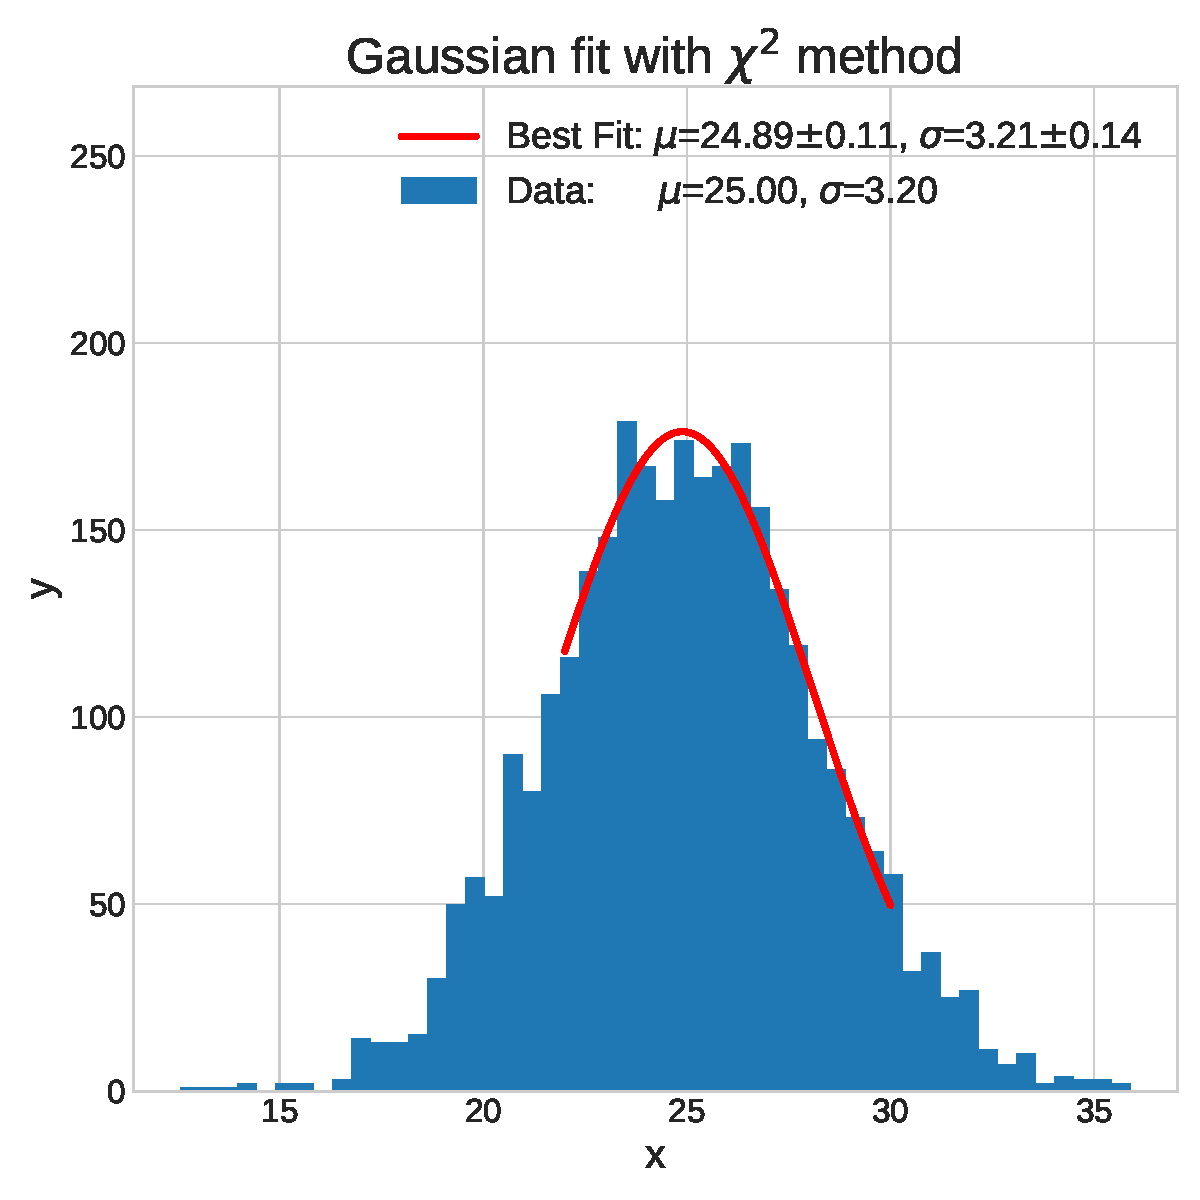
\includegraphics[width=0.45\textwidth]{exampleAnalysis/plots/Chi2_fit_MC.pdf}\\

\textbf{Ajustement des donn{\'e}es:}\\
\begin{align*}
G &= \mu_{\text{best}}/e = ... \\
\sigma_G &= \sigma_{\text{best}} / \mu_{\text{best}} = ...\%\\
\langle n_{\mathrm{pe}}\rangle &= ...
\end{align*}
\end{additional}
}

